\subsection{首达时及其应用}

\begin{definition}[首达时]
    首达时(first hitting time)定义为
    \begin{equation}
        V_A:=\min\{n\geq 0|X_n\in A\}
        \label{eq:FHT}
    \end{equation}
\end{definition}

注:前面提到的首次回访时间(first passage time)是要求 $n\geq 1$, rf. \eqref{eq:def_revisit_time}.

\subsubsection{击中概率(hitting time)与离出分布}

\begin{definition}[击中概率]
    击中概率定义为
    \begin{equation}
        h_x^A:=\PP_x(V_A<\infty)
        \label{eq:HT}
    \end{equation}
    特别地,$A$为闭集,称$h_x^A$为吸收概率
\end{definition}

下面介绍 $h_x^A$ 的一个性质

\begin{lemma}
    $h^A:=(h_x^A)_{x\in S}$ 满足下列方程
    \begin{equation}
\begin{cases}
        h_x^A=1 & x\in A\\
        h_x^A=\sum_y p_{xy}h_y^A & x\notin A
    \end{cases}
\end{equation}
    其中 $x\notin A$ 的情况对应卷积 $f(x)=(f*g)(x)=\sum_{y\in s}f(y)g(x-y)$.
\end{lemma}

击中概率是上述方程的一个解,之后我们将验证其唯一性.
\begin{proof}
$x\in A\Rightarrow V_A=0$, 所以 $h_x^A = \PP_x(V_A < \infty) = 1$.

$x\notin A\Rightarrow V_A\geq 1$, 考虑一步转移情况(one step reasoning) $\leftarrow$ 证明思想
\[
h_x^A=\sum_{y\in S}\PP_x(V_A<\infty, X_1=y)=\sum_{y\in S}\PP(V_A<\infty| X_1=y,X_0=x)\PP(X_1=y|X_0=x)
\]
\begin{claim}
$\PP(V_A<\infty|X_1=y,X_0=x)=h_y^A,\forall y\in S, x\notin A$
\end{claim}
利用马氏性,
\[
\begin{aligned}
    \PP(V_A<\infty| X_1=y,X_0=x) &\xlongequal{x\notin A}\PP(\bigcup_{n\geq 1}\{X_n\in A\}|X_1=y,X_0=x)\\
    &\xlongequal{\text{Markov}}\PP(\bigcup_{n\geq 1}\{X_n\in A\}|X_1=y)\\
    &\xlongequal{\text{SMP}}\PP_y(\bigcup_{n\geq 0}\{X_n\in A\})=\PP_y(V_A<\infty)=h_y^A
\end{aligned}
\]
\end{proof}

\begin{example}
    $a,b\in S,V_a:=V_{\{a\}},V_b:=V_{\{b\}}$, 考虑 $h(x)=\PP_x(V_a<V_b)$, 则 $h=(h(x))_{x\in S}$ 满足下列方程
    \[
    \begin{cases}
        h(a)=1, h(b)=0\\
        h(x)=\sum_y p_{xy}h(y) & x\neq a,b
    \end{cases}
    \]
\end{example}
\begin{proof}
(和上述引理证明过程一样) 使用一步展开方法, 
\[
h(x)=\PP_x(V_a<V_b)=\sum_{y\in S}\PP_x(V_a<V_b|X_1=y)\PP_x(X_1=y)
\]
只需证$\PP_x(V_a<V_b|X_1=y)=h(y),\forall x\neq a,b, y\in S, \to V_a\geq 1$, 就满足 $h(x)=\sum_{y\in S}p_{xy}h(y)$.
\[
\begin{aligned}
    \text{LHS} &=\PP_x(1\leq V_a<\infty, V_a<V_b|X_1=y)\\
    &\xlongequal{x\neq a,b}\PP_x\left(\bigcup_{m\geq 1}\left\{\{X_m=a\}\cap \bigcap_{1\leq k\leq m}\{X_k\neq a,b\}\right\}\bigg|X_1=y\right)\\
    &=\PP_x\left(\sum_{m\geq 1}\left\{\{X_m=a\}\cap \bigcap_{1\leq k\leq m}\{X_k\neq a,b\}\right\}\bigg|X_1=y\right)\\
    &=\sum_{m\geq 1}\PP_x\left(\{X_m=a\}\cap \bigcap_{1\leq k\leq m}\{X_k\neq a,b\}\bigg|X_1=y\right)\\
    &\xlongequal{\text{Markov}}\sum_{m\geq 1}\PP(V_a=m,V_a<V_b|X_1=y)\\
    &\xlongequal{\text{SMP}}\sum_{m\geq 1}\PP_y(V_a=m,V_a<V_b)\\
    &=\PP_y(V_a<V_b)=h(y)
\end{aligned}
\]
\end{proof}

\begin{theorem}\label{thm:fht-unique}
    $A,B\st S,A\cap B=\emp$, 令 $C=S-A\cup B$. 若 $C$ 有限, $\PP_x(V_A\land V_B<\infty)>0, \forall x\in C$, 则方程
    \begin{equation}
\begin{cases}
        h(x)=1 & x\in A\\
        h(x)=\sum_{y\in S}p_{xy}h(y) & x\in C\\
        h(x)=0 & x\in B
    \end{cases}
\end{equation}
    存在唯一非负解 $h(x)=\PP_x(V_A<V_B), \forall x\in S$ (不证明)
\end{theorem}

注:\begin{enumerate}
		\item $\land$ 是取小符号, $V_A\land V_B:=\min\{V_A,V_B \}$
    \item $\PP_x(V_a\land V_b<\infty)>0\iff x\to a \text{ 或 } x\to b$
    \item $A\cap B=\emp$ 时, $V_A\land V_B=V_{A\cup B}$
\end{enumerate}

\begin{problem}[作业8-1]
    证明:
    \begin{enumerate}
\item $\PP_x(V_a\land V_b<\infty)>0\iff x\to a \text{ 或 }x\to b$
\item $A\cap B=\emp$ 时, $V_A\land V_B=V_{A\cup B}$
\end{enumerate}
\end{problem}

\begin{figure}[H]
    \centering
    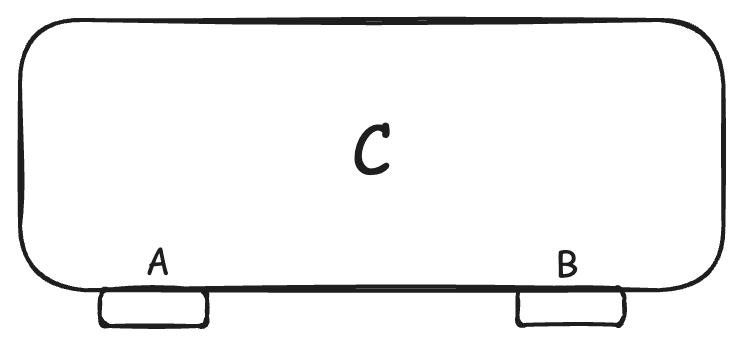
\includegraphics[width=0.35\textwidth]{figures/first-hitting.png}
    \caption{An example}
\end{figure}

$\tau_C=\min\{n\geq 0|X_n\notin C\}$ 为首次离出时刻/逃逸时刻.

$\tau=\min\{n\geq 0|X_n\in A\cup B\}, A\cap B=\emp$.

$\PP_x(X_{\tau_C}\in A)=\PP_x(V_A<V_B)$ 为逃逸概率/离出分布.

特别的, $A=\{a\}, B=\{b\}$, $a,b$ 为吸收态, $x\to a(x\neq a)$, $a\nrightarrow x, \rho_{ax}=0<1$, 由 Lem \ref{lem:commu_recurrent}, $x$ 暂留. 

$\PP_x(V_a<V_b)=\PP_x(V_a<\infty)$ 为吸收概率.

$\tau_C=V_{A\cup B}=V_A\land V_B$

$\therefore \PP_x(V_A\land V_B<\infty)=\PP_x(\tau_C<\infty)>0$.

\begin{example}\label{exa:1.43}
    $X_n$: 财富, $X_n=0$或$N$时游戏结束, 问: 赌徒破产概率.
\end{example}
\begin{proof}[解]
    \[
    \begin{cases}
        p(x,x+1)=p & 0<x<N\\
        p(x,x-1)=q=1-p & 0<x<N\\
        p(0,0)=1,p(N,N)=1 & x=0,x=N
    \end{cases}
    \]
    $0,N$ 为吸收态. 令 $h(x):=\PP_x(V_0<\infty)=\PP_x(V_0<V_N)$, $x=1,\cdots,N-1$. $S$ 有限, 不可约, 则 $\forall 0<x<N, x\to 0, x\to N$.
    \begin{figure}[H]
        \centering
        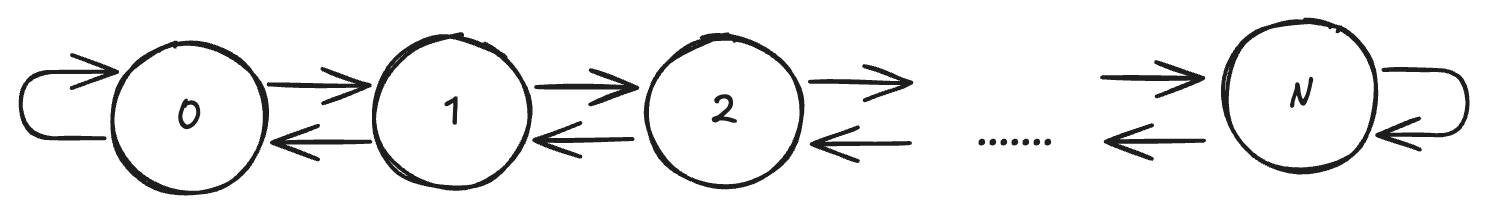
\includegraphics[width=0.55\textwidth]{figures/exa_p79.png}
    \end{figure}
    由 Thm \ref{thm:fht-unique}, $h(x)=(h(x))_{x\in S}$ 是下列方程的唯一非负解.
    \[
    \begin{cases}
        h(0)=1, h(N)=0\\
        h(x)=\sum_y p_{xy}h(y)=p(x,x+1)h(x+1)+p(x,x-1)h(x-1) & 0<x<N\\
    \end{cases}
    \]
    $h(x)=ph(x+1)+qh(x-1), 0<x<N$. $p(h(x+1)-h(x))=q(h(x)-h(x-1))$.
    \[
    h(x+1)-h(x)=\frac{q}{p}(h(x)-h(x-1))=\left(\frac{q}{p}\right)^x(h(1)-h(0)),\quad \forall 0\leq x\leq N
    \]
    \[
    \begin{aligned}
    h(x) &=h(0)+\sum_{k=0}^{x-1}(h(k+1)-h(k))\\
    &=h(0)+(h(1)-h(0))\sum_{k=0}^{x-1}\left(\frac{q}{p}\right)^x,\quad \forall 0\leq x\leq N
    \end{aligned}
    \]
    令 $\theta=q/p$.
\begin{enumerate}
    \item $\theta=1$ 时, $h(x)=h(0)+x(h(1)-h(0))$, $0=h(N)=1+N(h(1)-h(0))$, $h(1)-h(0)=-1/N$, $h(x)=1+(-1/N)x=(N-x)/N$
    \item $\theta\neq 1$ 时, 同理.
\end{enumerate}
\end{proof}
还有一种用线性代数方法求

$h[A]:=(h(x))_{x\in A}$ (列), $P[C,C]=(p_{ij})_{i,j\in C}$, $h(x)=\PP_x(V_A<V_B)$.
\[
\begin{cases}
h(x)=1 & x\in A\\
h(x)=0 & x\in B\\
h(x)=\sum_{y\in S}p_{xy}h(y) & x\in C
\end{cases}\Rightarrow 
\begin{cases}
    h[A]=\mathbf{1}\\
    h[B]=\mathbf{0}\\
    h[C]=P[C,C]h[C]+P[C,A]\mathbf{1}
\end{cases}
\]
因为 $A,B,C$ 互不相交, 
\[
\begin{aligned}
h(x)&=\sum_{y\in S}p_{xy}h(y)\\
&=\sum_{y\in A}p_{xy}h(y)+\sum_{y\in B}p_{xy}h(y)+\sum_{y\in C}p_{xy}h(y)\\
&=\sum_{y\in A}p_{xy}+\sum_{y\in C}p_{xy}h(y)\\
&=(P[x,A])_{x\in C}\mathbf{1}+(P[x,C])_{x\in C}(h(y))_{y\in C}\\
&=P[C,A]\mathbf{1}+P[C,C]h[C],\forall x\in C
\end{aligned}
\]
$\Rightarrow h[C]=(I_{|C|}-P[C,C])^{-1}P[C,A]\mathbf{1}$

\subsubsection{平均首达时与离出时刻}

\begin{definition}
    定义平均首达时.
    \[
    k_x^A:=\EE[V_A|X_0=x]=\begin{cases}
        \sum_{n\geq 0}n\PP_x(V_A=n) & \PP_x(V_A<\infty)=1\\
        \infty & \PP_x(V_A=\infty)>0
    \end{cases}
    \]
\end{definition}
\textcolor{red}{思考:} $\PP_x(V_A<\infty)=1$ 与常返的区别是? 

常返 $\PP_x(T_x<\infty)=1$ 是 $\PP_x(V_A<\infty)=1$ 的充分不必要条件.

\begin{lemma}
    $k^A=(k_x^A)_{x\in S}$ 满足
    \[
    \begin{cases}
        k_x^A=0 & x\in A\\
        k_x^A=1+\sum_{y\in S}p_{xy}k_y^A & x\notin A
    \end{cases}
    \]
\end{lemma}

\begin{proof}
当 $x\in A$ 时, $V_A=0, k_x^A=0$. 当 $x\notin A$ 时,
\[
\EE_x V_A=\sum_{y\in S}\EE_x[V_A\II_{\{X_1=y\}}]\xlongequal{\text{Cor }\eqref{cor:con_exp_indic}}\sum_{y\in S}\EE_x[V_A|X_1=y]\PP_x(X_1=y)
\]
\begin{claim}\label{claim:w8-hw2}
$\EE_x[V_A|X_1=y]=\EE[V_A+1|X_0=y], \forall y\in S, x\notin A$.
\end{claim}
\begin{proof}
见 HW Week8 作业2.
\end{proof}
将 Claim \ref{claim:w8-hw2} 代回 $\EE_x V_A$.
\[
\begin{aligned}
\sum_{y\in S}\EE_x[V_A|X_1=y]\PP_x(X_1=y)&=\sum_{y\in S}p_{xy}(1+\EE[V_A|X_0=y])\\
&=\sum_{y\in S}p_{xy}+\sum_{y\in S}p_{xy}k_y^A\\
&=1+\sum_{y\in S}p_{xy}k_y^A
\end{aligned}
\]
\end{proof}

\begin{theorem}\label{thm:p81}
    令 $C=S-A, A\st S$. 若 $C$ 有限, 且 $\forall x\in C, \PP_x(V_A<\infty)$=1. 则
    \begin{equation}
    \begin{cases}
        g(x)=0 & x\in A\\
        g(x)=1+\sum_{y\in C}p_{xy}g(y) & x\in C
    \end{cases}
    \end{equation}
    存在唯一非负解 $g(x)=\EE_xV_A$. 
\end{theorem}
$g[C]=\mathbf{1}+P[C,C]g[C]$. $g[C]=(I_{|C|}-P[C,C])^{-1}\mathbf{1}\overset{\text{书上}}{=}(\mathbf{I}-\mathbf{\gamma})^{-1}\mathbf{1}$

继续 Gambler's Ruin 例题

离出时刻 $\tau_C:=\min\{n\geq 0|X_n\neq C\}=V_{C^c}$

离出分布 $X_{\tau_C}$ 的分布
\begin{enumerate}
    \item $X_{\tau_C}\in C^c$, 故 $\{X_{\tau_C}=C^c\}=\Omega$
    \item 令 $x\in C,A\st C^c,\PP_x(X_{\tau_C}\in A)=\PP_x(V_A<V_{C^c})$
\end{enumerate}

\begin{example}[等待HT出现的时间]\label{exa:1.48}
    $X_n$: $n+1$ 时刻硬币朝上的图案, $n\geq 0$, $S_x=\{H,T\}$. 令 $Y_n=(X_n,X_{n+1}),n\geq 0$, 考虑其为马氏链且 $S=\{HH,HT,TH,TT\}$.
    \begin{align*}
        \mathbf{P}=~
        \bordermatrix{
        &\bf HH&\bf HT&\bf TH&\bf TT \cr
        \bf HH&0.5&0.5&0&0 \cr
        \bf HT&0&0&0.5&0.5 \cr
        \bf TH&0.5&0.5&0&0 \cr
        \bf TT&0&0&0.5&0.5 \cr
        }~
    \end{align*}
    令 $T_{HT}$ 为出现 $HT$ 所需的硬币投掷数. 求 $\EE T_{HT}$.
\end{example}

\begin{proof}[解]
    $A=\{HT\}, V_A:=\min\{n\geq 0|Y_n=(X_n,X_{n+1})\in A\}$, $T_{HT}=V_A+2$
    
    (Step 1) 求 $\EE_xV_A$. $S$ 有限, 不可约. 由 Thm \ref{thm:p81}, $g(x):=\EE_xV_A$ 是下列方程的唯一非负解.
    \[
    \begin{cases}
        g[A]=0\\
        g[C]=\mathbf{1}_{|C|}+P[C,C]g[C]
    \end{cases}
    \]
    \[
    g[C]=(I_{|C|}-P[C,C])^{-1}\mathbf{1}_{|C|}=\begin{bmatrix}
        2\\2\\4
    \end{bmatrix}\begin{matrix}
        \bf HH \\ \bf TH\\ \bf TT
    \end{matrix}
    \]
    (Step 2)
    \[
    \begin{aligned}
        \EE T_{HT}&=2+\EE V_A\\
        &=2+\sum_{x\in S}\EE V_A\II_{\{Y_0=x\}}\\
        &\xlongequal{\text{Cor }\eqref{cor:con_exp_indic}}2+\sum_{x\in S}\EE[V_A|Y_0=x]\PP(Y_0=x)\\
        &=2+\sum_{x\in S}g(x)\PP(X_0=H,X_1=T)\\
        &=2+\frac{1}{4}(0+2+2+4)=4
    \end{aligned}
    \]
\end{proof}
\newpage